% Options for packages loaded elsewhere
\PassOptionsToPackage{unicode}{hyperref}
\PassOptionsToPackage{hyphens}{url}
\PassOptionsToPackage{dvipsnames,svgnames,x11names}{xcolor}
%
\documentclass[
]{estat/estat}

\usepackage{amsmath,amssymb}
\usepackage{iftex}
\ifPDFTeX
  \usepackage[T1]{fontenc}
  \usepackage[utf8]{inputenc}
  \usepackage{textcomp} % provide euro and other symbols
\else % if luatex or xetex
  \usepackage{unicode-math}
  \defaultfontfeatures{Scale=MatchLowercase}
  \defaultfontfeatures[\rmfamily]{Ligatures=TeX,Scale=1}
\fi
\usepackage{lmodern}
\ifPDFTeX\else  
    % xetex/luatex font selection
    \setmainfont[]{Arial}
\fi
% Use upquote if available, for straight quotes in verbatim environments
\IfFileExists{upquote.sty}{\usepackage{upquote}}{}
\IfFileExists{microtype.sty}{% use microtype if available
  \usepackage[]{microtype}
  \UseMicrotypeSet[protrusion]{basicmath} % disable protrusion for tt fonts
}{}
\makeatletter
\@ifundefined{KOMAClassName}{% if non-KOMA class
  \IfFileExists{parskip.sty}{%
    \usepackage{parskip}
  }{% else
    \setlength{\parindent}{0pt}
    \setlength{\parskip}{6pt plus 2pt minus 1pt}}
}{% if KOMA class
  \KOMAoptions{parskip=half}}
\makeatother
\usepackage{xcolor}
\usepackage[left=3cm,right=2cm,top=3cm,bottom=2cm]{geometry}
\setlength{\emergencystretch}{3em} % prevent overfull lines
\setcounter{secnumdepth}{5}
% Make \paragraph and \subparagraph free-standing
\makeatletter
\ifx\paragraph\undefined\else
  \let\oldparagraph\paragraph
  \renewcommand{\paragraph}{
    \@ifstar
      \xxxParagraphStar
      \xxxParagraphNoStar
  }
  \newcommand{\xxxParagraphStar}[1]{\oldparagraph*{#1}\mbox{}}
  \newcommand{\xxxParagraphNoStar}[1]{\oldparagraph{#1}\mbox{}}
\fi
\ifx\subparagraph\undefined\else
  \let\oldsubparagraph\subparagraph
  \renewcommand{\subparagraph}{
    \@ifstar
      \xxxSubParagraphStar
      \xxxSubParagraphNoStar
  }
  \newcommand{\xxxSubParagraphStar}[1]{\oldsubparagraph*{#1}\mbox{}}
  \newcommand{\xxxSubParagraphNoStar}[1]{\oldsubparagraph{#1}\mbox{}}
\fi
\makeatother


\providecommand{\tightlist}{%
  \setlength{\itemsep}{0pt}\setlength{\parskip}{0pt}}\usepackage{longtable,booktabs,array}
\usepackage{calc} % for calculating minipage widths
% Correct order of tables after \paragraph or \subparagraph
\usepackage{etoolbox}
\makeatletter
\patchcmd\longtable{\par}{\if@noskipsec\mbox{}\fi\par}{}{}
\makeatother
% Allow footnotes in longtable head/foot
\IfFileExists{footnotehyper.sty}{\usepackage{footnotehyper}}{\usepackage{footnote}}
\makesavenoteenv{longtable}
\usepackage{graphicx}
\makeatletter
\def\maxwidth{\ifdim\Gin@nat@width>\linewidth\linewidth\else\Gin@nat@width\fi}
\def\maxheight{\ifdim\Gin@nat@height>\textheight\textheight\else\Gin@nat@height\fi}
\makeatother
% Scale images if necessary, so that they will not overflow the page
% margins by default, and it is still possible to overwrite the defaults
% using explicit options in \includegraphics[width, height, ...]{}
\setkeys{Gin}{width=\maxwidth,height=\maxheight,keepaspectratio}
% Set default figure placement to htbp
\makeatletter
\def\fps@figure{htbp}
\makeatother

\authors{%
    Bruno Boaventura Xavier\\

    
}

% escreva o nome do cliente aqui
% se for mais de um separe por \\
\client{%
    House of Excellence
}
% Baixando pacotes
\RequirePackage{fancyhdr}
\RequirePackage{graphicx}

\setlength\headheight{28pt}  

\setlength{\parindent}{15pt} % Adiciona indentação nos parágrafos
\setlength{\parskip}{0pt} % Adiciona 0 espaço entro os parágrafos

\newcommand{\estat}{\textbf{ESTAT}\xspace}
\newcommand{\direx}{\textbf{DIREX}\xspace}
\makeatletter
\@ifpackageloaded{caption}{}{\usepackage{caption}}
\AtBeginDocument{%
\ifdefined\contentsname
  \renewcommand*\contentsname{Índice}
\else
  \newcommand\contentsname{Índice}
\fi
\ifdefined\listfigurename
  \renewcommand*\listfigurename{Lista de Figuras}
\else
  \newcommand\listfigurename{Lista de Figuras}
\fi
\ifdefined\listtablename
  \renewcommand*\listtablename{Lista de Tabelas}
\else
  \newcommand\listtablename{Lista de Tabelas}
\fi
\ifdefined\figurename
  \renewcommand*\figurename{Figura}
\else
  \newcommand\figurename{Figura}
\fi
\ifdefined\tablename
  \renewcommand*\tablename{Tabela}
\else
  \newcommand\tablename{Tabela}
\fi
}
\@ifpackageloaded{float}{}{\usepackage{float}}
\floatstyle{ruled}
\@ifundefined{c@chapter}{\newfloat{codelisting}{h}{lop}}{\newfloat{codelisting}{h}{lop}[chapter]}
\floatname{codelisting}{Listagem}
\newcommand*\listoflistings{\listof{codelisting}{Lista de Listagens}}
\captionsetup{labelsep=colon}
\makeatother
\makeatletter
\makeatother
\makeatletter
\@ifpackageloaded{caption}{}{\usepackage{caption}}
\@ifpackageloaded{subcaption}{}{\usepackage{subcaption}}
\makeatother

\ifLuaTeX
\usepackage[bidi=basic]{babel}
\else
\usepackage[bidi=default]{babel}
\fi
\babelprovide[main,import]{portuguese}
\ifPDFTeX
\else
\babelfont{rm}[]{Arial}
\fi
% get rid of language-specific shorthands (see #6817):
\let\LanguageShortHands\languageshorthands
\def\languageshorthands#1{}
\ifLuaTeX
  \usepackage{selnolig}  % disable illegal ligatures
\fi
\usepackage{bookmark}

\IfFileExists{xurl.sty}{\usepackage{xurl}}{} % add URL line breaks if available
\urlstyle{same} % disable monospaced font for URLs
\hypersetup{
  pdftitle={Projeto - Fantasma},
  pdflang={pt},
  colorlinks=true,
  linkcolor={black},
  filecolor={black},
  citecolor={black},
  urlcolor={black},
  pdfcreator={LaTeX via pandoc}}


\title{Projeto - Fantasma}
\author{}
\date{}

\begin{document}
\maketitle

% Limpando tudo
\fancyhf{} 

% Ajustes do header
\fancyhead[L]{} % limpando o lado esquerdo
\fancyhead[R]{
\includegraphics[width=0.20\textwidth]{estat/imagens/estat.png}} % adicionando logo no canto direito
\renewcommand{\headrulewidth}{0pt}   % sem linha embaixo da logo

% Ajustes de fim de página
\fancyfoot[R]{\textcolor{white}{\thepage}} % Número em branco no canto direito

% Aplicando o estilo que acabamos de criar
\pagestyle{fancy} 

\renewcommand*\contentsname{Sumário}
{
\hypersetup{linkcolor=}
\setcounter{tocdepth}{3}
\tableofcontents
}

\section{Análises}\label{anuxe1lises}

\subsection{Top 5 países com mais medalhistas
femininas}\label{top-5-pauxedses-com-mais-medalhistas-femininas}

A partir do acesso ao banco de dados disponibilizado pela ``House of
Excellence'', tivemos acesso aos dados de todos os atletas que
participaram das olimpíadas de 2000 até 2016. Nesse cenário, com o
intuito de produzir um ranqueamento das cinco delegações que obtiveram
mais conquistas nesse período nas modalidades femininas, do banco de
dados original, foram utilizadas as variáveis de sexo(``Gender''), a
qual era dividida entre Feminino (``F'') e Masculino (``M''), ainda foi
utilizada a variável que descrevia qual país era a origem do atleta,
sendo a base para agrupar as conquistas, e por último a que evidenciava
qual medalha havia sido conquistada.

\begin{figure}

\caption{\label{fig-prop}Gráfico de colunas do total de conquistas de
cada delegação do Top 5}

\centering{

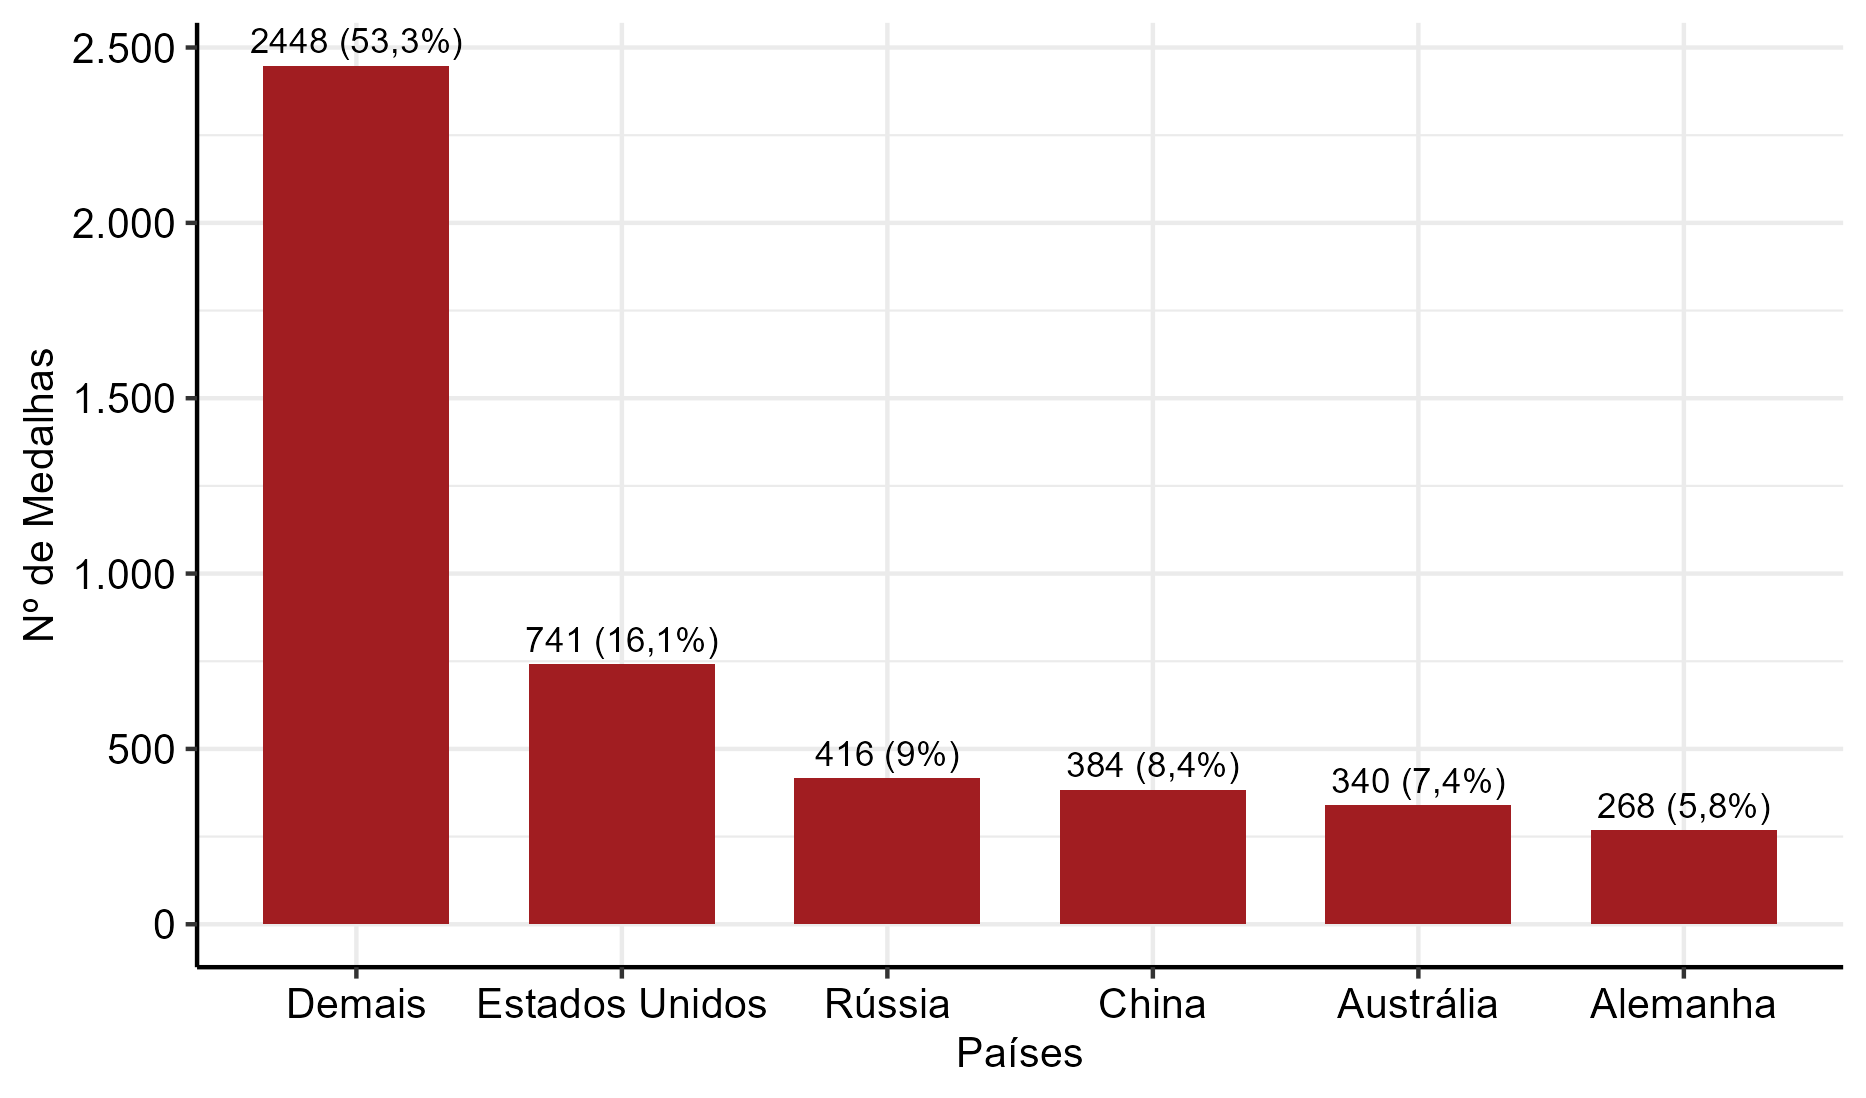
\includegraphics[width=158mm,height=\textheight]{images/colunas-prop-medalha.png}

}

\end{figure}%

Tendo a \ref{fig-prop} como referência podemos analisar que os Estados
Unidos lideram a lista com 741 medalhas, seguidos da delegação russa com
416 - o que representa uma diferença de 325 conquistas entre o primeiro
e o segundo colocado - em terceiro colocado está a China com 384, a
Austrália na quarta posição com 340 e fechando o ranqueamento a Alemanha
com 268, distanciando-se do penúltimo colocado por 72 medalhas e em
relação ao primeiro são 473 - valor maior que as conquistas da Rússia
que ocupa o segundo lugar.

Através da análise dos dados evidencia-se que dentre as modalidades
femininas, durante os anos de 2000 a 2016 considerando todas os pódios
sem distinção entre ouro, prata e bronze, totalizam-se 4597 conquistas.
Dado o interesse da ``House of Excelence'' em entender o cenário das
conquistas olímpicas, foi contruída uma análise da frequência dessas
medalhas em relação ao total de medalhas femininas. Assim por meio da
\ref{fig-prop}, no ``Top 5'' percebe-se que os Estados Unidos detém o
topo do quadro de medalhas com 16,12\%, seguido da Rússia que contém
9,05\% , a China em terceiro com 8,,35\%, a Austrália na quarta posição
com 7,4\% e fechando o ranqueamento a Alemanha com 5,83\%.

\begin{figure}[H]

\caption{\label{fig-setor}Gráfico de setor da frequência de conquistas
entre as delegações dentro e fora do Top 5}

\centering{

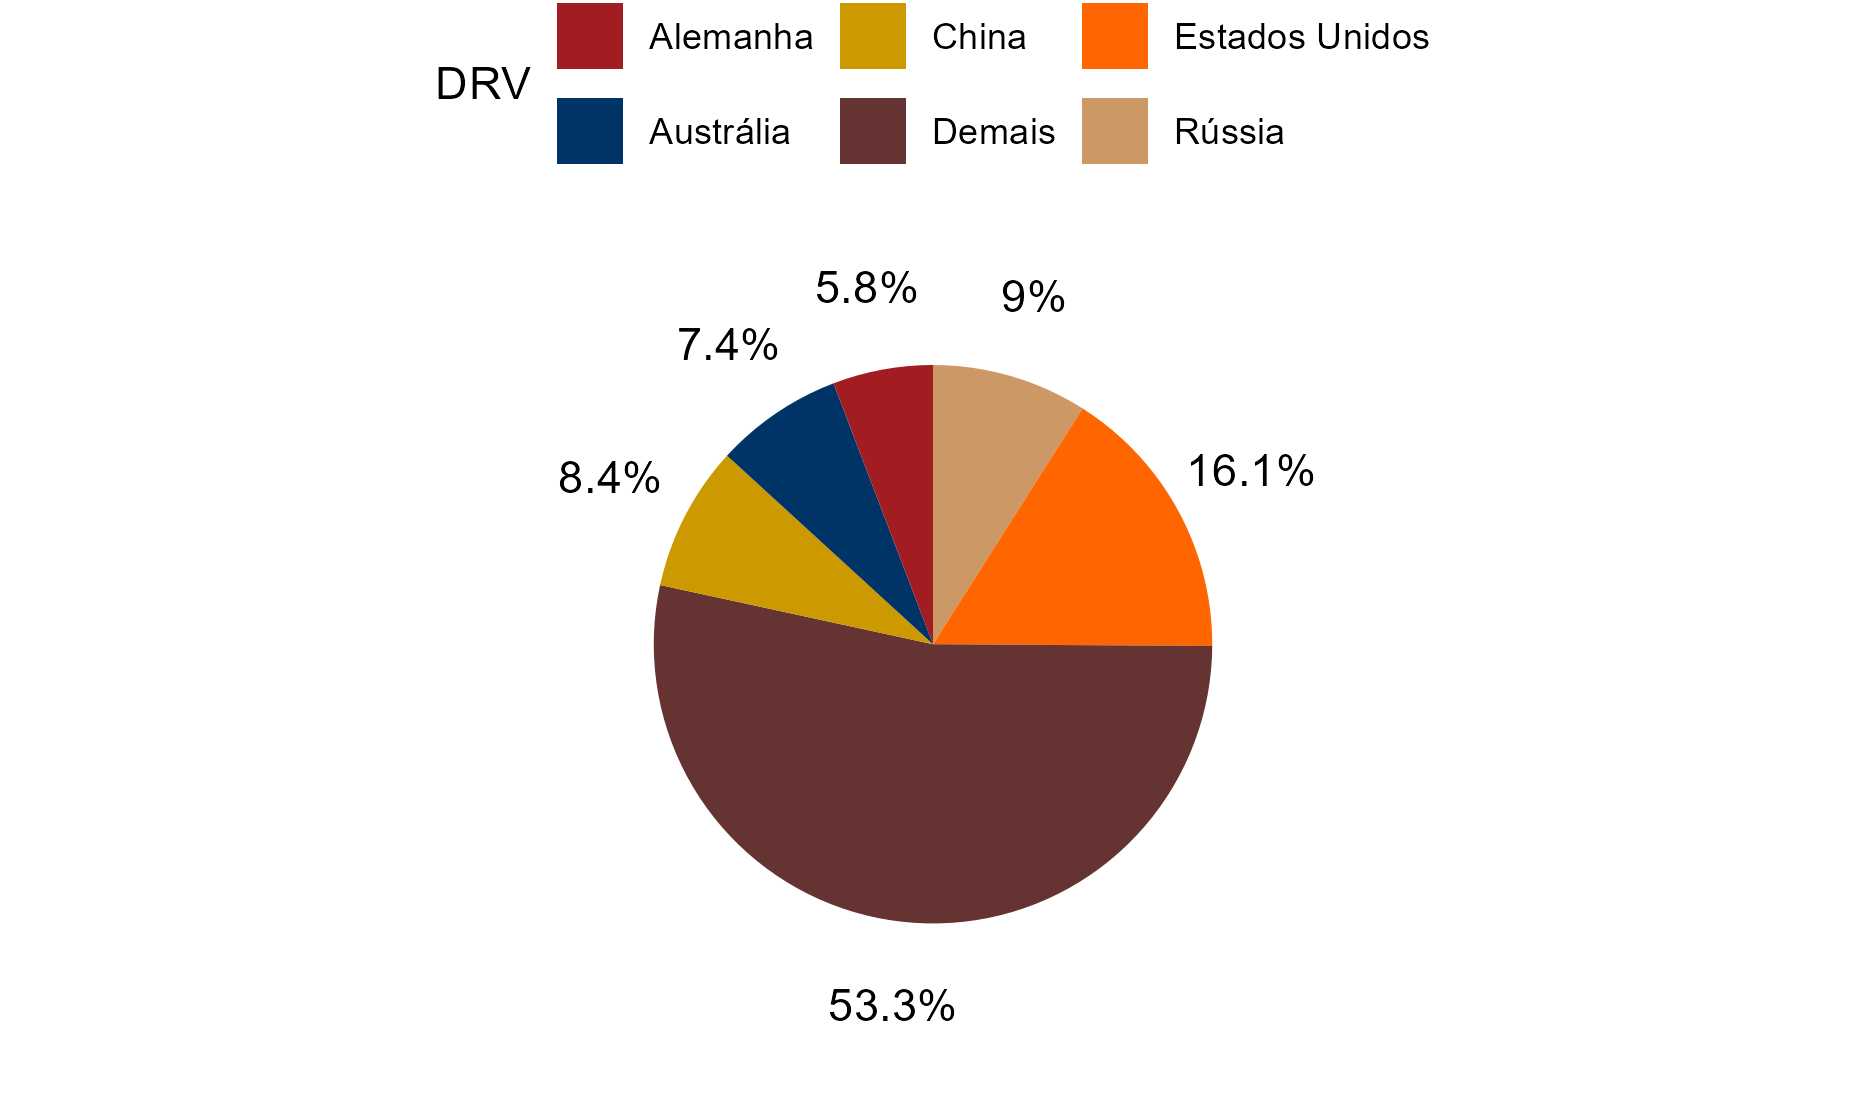
\includegraphics[width=158mm,height=\textheight]{images/setor_paises.png}

}

\end{figure}%

Para mais, a fim de esclarecer como os melhores países se comparam aos
demais, diante da \ref{fig-prop} e da \ref{fig-setor} analisa-se que as
delagações fora do ``Top 5'', totalizam 2448 pódios, o que representa
53,25\% do todo. Nesse cenário, nota-se que os cinco países com melhor
perfomance nos jogos possuem 2149 medalhas, o que condiz a 46,75\% de
todas as conquistas.




\end{document}
